% !TeX document-id = {8c6be429-7d79-4ce7-90ca-06d13b6696e5}
% !TeX TXS-program:bibliography = txs:///biber
\documentclass[14pt, russian]{scrartcl}
\let\counterwithout\relax
\let\counterwithin\relax
%\usepackage{lmodern}
\usepackage{float}
\usepackage{xcolor}
\usepackage{extsizes}
\usepackage{subfig}
\usepackage[export]{adjustbox}
\usepackage{tocvsec2} % возможность менять учитываемую глубину разделов в оглавлении
\usepackage[subfigure]{tocloft}
\usepackage[newfloat]{minted}
\setminted[text]{frame=single,fontsize = \footnotesize, linenos, xleftmargin = 1.5em, breaklines}
\setminted[rust]{frame=single,fontsize = \footnotesize, linenos, xleftmargin = 1.5em, breaklines}
\setminted[yaml]{frame=single,fontsize = \footnotesize, linenos, xleftmargin = 1.5em, breaklines}
\setminted[python]{frame=single,fontsize = \footnotesize, linenos, xleftmargin = 1.5em, breaklines}
\AtBeginEnvironment{figure}{\vspace{0.5cm}}
\AtBeginEnvironment{table}{\vspace{0.5cm}}
\AtBeginEnvironment{listing}{\vspace{0.5cm}}
\AtBeginEnvironment{minted}{\vspace{-0.5cm}}
\newenvironment{longlisting}{\captionsetup{type=listing}}{}
%\AfterEndEnvironment{minted}{\vspace{-1cm}}
\captionsetup[listing]{position=top}
\usepackage{array}
\usepackage{fancyvrb}
\usepackage{ulem,bm,mathrsfs,ifsym} %зачеркивания, особо жирный стиль и RSFS начертание
\usepackage{sectsty} % переопределение стилей подразделов
%%%%%%%%%%%%%%%%%%%%%%%

\newcolumntype{C}{>{\centering\arraybackslash}m{5em}}

%%% Поля и разметка страницы %%%
\usepackage{pdflscape}                              % Для включения альбомных страниц
\usepackage{geometry}                               % Для последующего задания полей
\geometry{a4paper,tmargin=2cm,bmargin=2cm,lmargin=3cm,rmargin=1cm} % тоже самое, но лучше
\newcommand*\lsin{\lstinline[columns=fixed]}

%%% Математические пакеты %%%
\usepackage{amsthm,amsfonts,amsmath,amssymb,amscd}  % Математические дополнения от AMS
\usepackage{mathtools}                              % Добавляет окружение multlined
\usepackage[perpage]{footmisc}
%\usepackage{times}

%%%% Установки для размера шрифта 14 pt %%%%
%% Формирование переменных и констант для сравнения (один раз для всех подключаемых файлов)%%
%% должно располагаться до вызова пакета fontspec или polyglossia, потому что они сбивают его работу
%\newlength{\curtextsize}
%\newlength{\bigtextsize}
%\setlength{\bigtextsize}{13pt}
\KOMAoptions{fontsize=14pt}

\makeatletter
\def\showfontsize{\f@size{} point}
\makeatother

%\makeatletter
%\show\f@size                                       % неплохо для отслеживания, но вызывает стопорение процесса, если документ компилируется без команды  -interaction=nonstopmode 
%\setlength{\curtextsize}{\f@size pt}
%\makeatother

%шрифт times
\usepackage{tempora}
%\usepackage{pscyr}
%\setmainfont[Ligatures={TeX,Historic}]{Times New Roman}

   %%% Решение проблемы копирования текста в буфер кракозябрами
%    \input glyphtounicode.tex
%    \input glyphtounicode-cmr.tex %from pdfx package
%    \pdfgentounicode=1
    \usepackage{cmap}                               % Улучшенный поиск русских слов в полученном pdf-файле
    \usepackage[T1]{fontenc}                       % Поддержка русских букв
    \usepackage[utf8]{inputenc}                     % Кодировка utf8
    \usepackage[english, main=russian]{babel}            % Языки: русский, английский
%   \IfFileExists{pscyr.sty}{\usepackage{pscyr}}{}  % Красивые русские шрифты
%\renewcommand{\rmdefault}{ftm}
%%% Оформление абзацев %%%
\usepackage{indentfirst}                            % Красная строка
%\usepackage{eskdpz}

%%% Таблицы %%%
\usepackage{longtable}                              % Длинные таблицы
\usepackage{multirow,makecell,array}                % Улучшенное форматирование таблиц
\usepackage{booktabs}                               % Возможность оформления таблиц в классическом книжном стиле (при правильном использовании не противоречит ГОСТ)

%%% Общее форматирование
\usepackage{soulutf8}                               % Поддержка переносоустойчивых подчёркиваний и зачёркиваний
\usepackage{icomma}                                 % Запятая в десятичных дробях



%%% Изображения %%%
\usepackage{graphicx}                               % Подключаем пакет работы с графикой
\graphicspath{{./images}}
\usepackage{wrapfig}

%%% Списки %%%
\usepackage{enumitem}

%%% Подписи %%%
\usepackage{caption}                                % Для управления подписями (рисунков и таблиц) % Может управлять номерами рисунков и таблиц с caption %Иногда может управлять заголовками в списках рисунков и таблиц
%% Использование:
%\begin{table}[h!]\ContinuedFloat - чтобы не переключать счетчик
%\captionsetup{labelformat=continued}% должен стоять до самого caption
%\caption{}
% либо ручками \caption*{Продолжение таблицы~\ref{...}.} :)

%%% Интервалы %%%
\addto\captionsrussian{%
  \renewcommand{\listingname}{Листинг}%
}
%%% Счётчики %%%
\usepackage[figure,table,section]{totalcount}               % Счётчик рисунков и таблиц
\DeclareTotalCounter{lstlisting}
\usepackage{totcount}                               % Пакет создания счётчиков на основе последнего номера подсчитываемого элемента (может требовать дважды компилировать документ)
\usepackage{totpages}                               % Счётчик страниц, совместимый с hyperref (ссылается на номер последней страницы). Желательно ставить последним пакетом в преамбуле

%%% Продвинутое управление групповыми ссылками (пока только формулами) %%%
%% Кодировки и шрифты %%%

%   \newfontfamily{\cyrillicfont}{Times New Roman}
%   \newfontfamily{\cyrillicfonttt}{CMU Typewriter Text}
	%\setmainfont{Times New Roman}
	%\newfontfamily\cyrillicfont{Times New Roman}
	%\setsansfont{Times New Roman}                    %% задаёт шрифт без засечек
%	\setmonofont{Liberation Mono}               %% задаёт моноширинный шрифт
%    \IfFileExists{pscyr.sty}{\renewcommand{\rmdefault}{ftm}}{}
%%% Интервалы %%%
%linespread-реализация ближе к реализации полуторного интервала в ворде.
%setspace реализация заточена под шрифты 10, 11, 12pt, под остальные кегли хуже, но всё же ближе к типографской классике. 
\linespread{1.3}                    % Полуторный интервал (ГОСТ Р 7.0.11-2011, 5.3.6)
%\renewcommand{\@biblabel}[1]{#1}

%%% Гиперссылки %%%
\usepackage{hyperref}

%%% Выравнивание и переносы %%%
\sloppy                             % Избавляемся от переполнений
\clubpenalty=10000                  % Запрещаем разрыв страницы после первой строки абзаца
\widowpenalty=10000                 % Запрещаем разрыв страницы после последней строки абзаца

\makeatletter % малые заглавные, small caps shape
\let\@@scshape=\scshape
\renewcommand{\scshape}{%
  \ifnum\strcmp{\f@series}{bx}=\z@
    \usefont{T1}{cmr}{bx}{sc}%
  \else
    \ifnum\strcmp{\f@shape}{it}=\z@
      \fontshape{scsl}\selectfont
    \else
      \@@scshape
    \fi
  \fi}
\makeatother

%%% Подписи %%%
%\captionsetup{%
%singlelinecheck=off,                % Многострочные подписи, например у таблиц
%skip=2pt,                           % Вертикальная отбивка между подписью и содержимым рисунка или таблицы определяется ключом
%justification=centering,            % Центрирование подписей, заданных командой \caption
%}
%%%        Подключение пакетов                 %%%
\usepackage{ifthen}                 % добавляет ifthenelse
%%% Инициализирование переменных, не трогать!  %%%
\newcounter{intvl}
\newcounter{otstup}
\newcounter{contnumeq}
\newcounter{contnumfig}
\newcounter{contnumtab}
\newcounter{pgnum}
\newcounter{bibliosel}
\newcounter{chapstyle}
\newcounter{headingdelim}
\newcounter{headingalign}
\newcounter{headingsize}
\newcounter{tabcap}
\newcounter{tablaba}
\newcounter{tabtita}
%%%%%%%%%%%%%%%%%%%%%%%%%%%%%%%%%%%%%%%%%%%%%%%%%%

%%% Область упрощённого управления оформлением %%%

%% Интервал между заголовками и между заголовком и текстом
% Заголовки отделяют от текста сверху и снизу тремя интервалами (ГОСТ Р 7.0.11-2011, 5.3.5)
\setcounter{intvl}{3}               % Коэффициент кратности к размеру шрифта

%% Отступы у заголовков в тексте
\setcounter{otstup}{0}              % 0 --- без отступа; 1 --- абзацный отступ

%% Нумерация формул, таблиц и рисунков
\setcounter{contnumeq}{1}           % Нумерация формул: 0 --- пораздельно (во введении подряд, без номера раздела); 1 --- сквозная нумерация по всей диссертации
\setcounter{contnumfig}{1}          % Нумерация рисунков: 0 --- пораздельно (во введении подряд, без номера раздела); 1 --- сквозная нумерация по всей диссертации
\setcounter{contnumtab}{1}          % Нумерация таблиц: 0 --- пораздельно (во введении подряд, без номера раздела); 1 --- сквозная нумерация по всей диссертации

%% Оглавление
\setcounter{pgnum}{0}               % 0 --- номера страниц никак не обозначены; 1 --- Стр. над номерами страниц (дважды компилировать после изменения)

%% Библиография
\setcounter{bibliosel}{1}           % 0 --- встроенная реализация с загрузкой файла через движок bibtex8; 1 --- реализация пакетом biblatex через движок biber

%% Текст и форматирование заголовков
\setcounter{chapstyle}{1}           % 0 --- разделы только под номером; 1 --- разделы с названием "Глава" перед номером
\setcounter{headingdelim}{1}        % 0 --- номер отделен пропуском в 1em или \quad; 1 --- номера разделов и приложений отделены точкой с пробелом, подразделы пропуском без точки; 2 --- номера разделов, подразделов и приложений отделены точкой с пробелом.

%% Выравнивание заголовков в тексте
\setcounter{headingalign}{0}        % 0 --- по центру; 1 --- по левому краю

%% Размеры заголовков в тексте
\setcounter{headingsize}{0}         % 0 --- по ГОСТ, все всегда 14 пт; 1 --- пропорционально изменяющийся размер в зависимости от базового шрифта

%% Подпись таблиц
\setcounter{tabcap}{0}              % 0 --- по ГОСТ, номер таблицы и название разделены тире, выровнены по левому краю, при необходимости на нескольких строках; 1 --- подпись таблицы не по ГОСТ, на двух и более строках, дальнейшие настройки: 
%Выравнивание первой строки, с подписью и номером
\setcounter{tablaba}{2}             % 0 --- по левому краю; 1 --- по центру; 2 --- по правому краю
%Выравнивание строк с самим названием таблицы
\setcounter{tabtita}{1}             % 0 --- по левому краю; 1 --- по центру; 2 --- по правому краю

%%% Рисунки %%%
\DeclareCaptionLabelSeparator*{emdash}{~--- }             % (ГОСТ 2.105, 4.3.1)
\captionsetup[figure]{labelsep=emdash,font=onehalfspacing,position=bottom}

%%% Таблицы %%%
\ifthenelse{\equal{\thetabcap}{0}}{%
    \newcommand{\tabcapalign}{\raggedright}  % по левому краю страницы или аналога parbox
}

\ifthenelse{\equal{\thetablaba}{0} \AND \equal{\thetabcap}{1}}{%
    \newcommand{\tabcapalign}{\raggedright}  % по левому краю страницы или аналога parbox
}

\ifthenelse{\equal{\thetablaba}{1} \AND \equal{\thetabcap}{1}}{%
    \newcommand{\tabcapalign}{\centering}    % по центру страницы или аналога parbox
}

\ifthenelse{\equal{\thetablaba}{2} \AND \equal{\thetabcap}{1}}{%
    \newcommand{\tabcapalign}{\raggedleft}   % по правому краю страницы или аналога parbox
}

\ifthenelse{\equal{\thetabtita}{0} \AND \equal{\thetabcap}{1}}{%
    \newcommand{\tabtitalign}{\raggedright}  % по левому краю страницы или аналога parbox
}

\ifthenelse{\equal{\thetabtita}{1} \AND \equal{\thetabcap}{1}}{%
    \newcommand{\tabtitalign}{\centering}    % по центру страницы или аналога parbox
}

\ifthenelse{\equal{\thetabtita}{2} \AND \equal{\thetabcap}{1}}{%
    \newcommand{\tabtitalign}{\raggedleft}   % по правому краю страницы или аналога parbox
}

\DeclareCaptionFormat{tablenocaption}{\tabcapalign #1\strut}        % Наименование таблицы отсутствует
\ifthenelse{\equal{\thetabcap}{0}}{%
    \DeclareCaptionFormat{tablecaption}{\tabcapalign #1#2#3}
    \captionsetup[table]{labelsep=emdash}                       % тире как разделитель идентификатора с номером от наименования
}{%
    \DeclareCaptionFormat{tablecaption}{\tabcapalign #1#2\par%  % Идентификатор таблицы на отдельной строке
        \tabtitalign{#3}}                                       % Наименование таблицы строкой ниже
    \captionsetup[table]{labelsep=space}                        % пробельный разделитель идентификатора с номером от наименования
}
\captionsetup[table]{format=tablecaption,singlelinecheck=off,font=onehalfspacing,position=top,skip=-5pt}  % многострочные наименования и прочее
\DeclareCaptionLabelFormat{continued}{Продолжение таблицы~#2}
\setlength{\belowcaptionskip}{.2cm}
\setlength{\intextsep}{0ex}

%%% Подписи подрисунков %%%
\renewcommand{\thesubfigure}{\asbuk{subfigure}}           % Буквенные номера подрисунков
\captionsetup[subfigure]{font={normalsize},               % Шрифт подписи названий подрисунков (не отличается от основного)
    labelformat=brace,                                    % Формат обозначения подрисунка
    justification=centering,                              % Выключка подписей (форматирование), один из вариантов            
}
%\DeclareCaptionFont{font12pt}{\fontsize{12pt}{13pt}\selectfont} % объявляем шрифт 12pt для использования в подписях, тут же надо интерлиньяж объявлять, если не наследуется
%\captionsetup[subfigure]{font={font12pt}}                 % Шрифт подписи названий подрисунков (всегда 12pt)

%%% Настройки гиперссылок %%%

\definecolor{linkcolor}{rgb}{0.0,0,0}
\definecolor{citecolor}{rgb}{0,0.0,0}
\definecolor{urlcolor}{rgb}{0,0,0}

\hypersetup{
    linktocpage=true,           % ссылки с номера страницы в оглавлении, списке таблиц и списке рисунков
%    linktoc=all,                % both the section and page part are links
%    pdfpagelabels=false,        % set PDF page labels (true|false)
    plainpages=true,           % Forces page anchors to be named by the Arabic form  of the page number, rather than the formatted form
    colorlinks,                 % ссылки отображаются раскрашенным текстом, а не раскрашенным прямоугольником, вокруг текста
    linkcolor={linkcolor},      % цвет ссылок типа ref, eqref и подобных
    citecolor={citecolor},      % цвет ссылок-цитат
    urlcolor={urlcolor},        % цвет гиперссылок
    pdflang={ru},
}
\urlstyle{same}
%%% Шаблон %%%
%\DeclareRobustCommand{\todo}{\textcolor{red}}       % решаем проблему превращения названия цвета в результате \MakeUppercase, http://tex.stackexchange.com/a/187930/79756 , \DeclareRobustCommand protects \todo from expanding inside \MakeUppercase
\setlength{\parindent}{2.5em}                       % Абзацный отступ. Должен быть одинаковым по всему тексту и равен пяти знакам (ГОСТ Р 7.0.11-2011, 5.3.7).

%%% Списки %%%
% Используем дефис для ненумерованных списков (ГОСТ 2.105-95, 4.1.7)
%\renewcommand{\labelitemi}{\normalfont\bfseries~{---}} 
\renewcommand{\labelitemi}{\bfseries~{---}} 
\setlist{nosep,%                                    % Единый стиль для всех списков (пакет enumitem), без дополнительных интервалов.
    labelindent=\parindent,leftmargin=*%            % Каждый пункт, подпункт и перечисление записывают с абзацного отступа (ГОСТ 2.105-95, 4.1.8)
}
%%%%%%%%%%%%%%%%%%%%%%
%\usepackage{xltxtra} % load xunicode

\usepackage{ragged2e}
\usepackage[explicit]{titlesec}
\usepackage{placeins}
\usepackage{xparse}
\usepackage{csquotes}

\usepackage{listingsutf8}
\usepackage{url} %пакеты расширений
\usepackage{algorithm}
\usepackage[noend]{algpseudocode}
\usepackage{blkarray}
\usepackage{chngcntr}
\usepackage{tabularx}
\usepackage[backend=biber, 
    maxnames=5,
    bibstyle=gost-numeric,
    citestyle=nature]{biblatex}
\newcommand*\template[1]{\text{<}#1\text{>}}
\addbibresource{biblio.bib}
\renewcommand{\mkgostheading}[1]{#1}
\renewcommand*{\newblockpunct}{\addperiod\addnbspace\textendash\space\bibsentence}
\renewcommand*{\bibrangedash}{\text{\textendash}}
\titleformat{name=\section,numberless}[block]{\normalfont\Large\centering}{}{0em}{#1}
\titleformat{\section}[block]{\normalfont\Large\bfseries\raggedright}{}{0em}{\thesection\hspace{0.25em}#1}
\titleformat{\subsection}[block]{\normalfont\Large\bfseries\raggedright}{}{0em}{\thesubsection\hspace{0.25em}#1}
\titleformat{\subsubsection}[block]{\normalfont\large\bfseries\raggedright}{}{0em}{\thesubsubsection\hspace{0.25em}#1}

\let\Algorithm\algorithm
\renewcommand\algorithm[1][]{\Algorithm[#1]\setstretch{1.5}}
%\renewcommand{\listingscaption}{Листинг}

\usepackage{pifont}
\usepackage{calc}
\usepackage{suffix}
\usepackage[none]{hyphenat}
\usepackage{csquotes}
\DeclareQuoteStyle{russian}
    {\guillemotleft}{\guillemotright}[0.025em]
    {\quotedblbase}{\textquotedblleft}
\ExecuteQuoteOptions{style=russian}
\newcommand{\enq}[1]{\enquote{#1}}  
\newcommand{\eng}[1]{\begin{english}#1\end{english}}
% Подчиненные счетчики в окружениях http://old.kpfu.ru/journals/izv_vuz/arch/sample1251.tex
\newcounter{cTheorem} 
\newcounter{cDefinition}
\newcounter{cConsequent}
\newcounter{cExample}
\newcounter{cLemma}
\newcounter{cConjecture}
\newtheorem{Theorem}{Теорема}[cTheorem]
\newtheorem{Definition}{Определение}[cDefinition]
\newtheorem{Consequent}{Следствие}[cConsequent]
\newtheorem{Example}{Пример}[cExample]
\newtheorem{Lemma}{Лемма}[cLemma]
\newtheorem{Conjecture}{Гипотеза}[cConjecture]

\renewcommand{\theTheorem}{\arabic{Theorem}}
\renewcommand{\theDefinition}{\arabic{Definition}}
\renewcommand{\theConsequent}{\arabic{Consequent}}
\renewcommand{\theExample}{\arabic{Example}}
\renewcommand{\theLemma}{\arabic{Lemma}}
\renewcommand{\theConjecture}{\arabic{Conjecture}}
%\makeatletter
\NewDocumentCommand{\Newline}{}{\text{\\}}
\newcommand{\sequence}[2]{\ensuremath \left(#1,\ \dots,\ #2\right)}

\definecolor{mygreen}{rgb}{0,0.6,0}
\definecolor{mygray}{rgb}{0.5,0.5,0.5}
\definecolor{mymauve}{rgb}{0.58,0,0.82}
\renewcommand{\listalgorithmname}{Список алгоритмов}
\floatname{algorithm}{Листинг}



\renewcommand{\lstlistingname}{Листинг}
\DeclareCaptionFormat{listing}{#1 --- #3}
\captionsetup[listing]{format=listing, singlelinecheck=false, labelsep=colon}




\renewcommand{\thealgorithm}{\arabic{algorithm}}

\newcommand{\refAlgo}[1]{(листинг \ref{#1})}
\newcommand{\refImage}[1]{(рисунок \ref{#1})}

\renewcommand{\theenumi}{\arabic{enumi}.}% Меняем везде перечисления на цифра.цифра	
\renewcommand{\labelenumi}{\arabic{enumi}.}% Меняем везде перечисления на цифра.цифра
\renewcommand{\theenumii}{\arabic{enumii}}% Меняем везде перечисления на цифра.цифра
\renewcommand{\labelenumii}{(\arabic{enumii})}% Меняем везде перечисления на цифра.цифра
\renewcommand{\theenumiii}{\roman{enumiii}}% Меняем везде перечисления на цифра.цифра
\renewcommand{\labelenumiii}{(\roman{enumiii})}% Меняем везде перечисления на цифра.цифра
%\newfontfamily\AnkaCoder[Path=src/fonts/]{AnkaCoder-r.ttf}
\renewcommand{\labelitemi}{---}
\renewcommand{\labelitemii}{---}

\def\customfigurename{Рисунок}
% Define a new counter for the custom figures
\newcounter{customfigurecounter}
\renewcommand{\thecustomfigurecounter}{A.\arabic{customfigurecounter}}

% Define a new float environment for the custom figures
\DeclareFloatingEnvironment[fileext=cust]{customfigure}

% Redefine the caption format for the custom figures
\DeclareCaptionLabelFormat{customlabel}{#1~\thecustomfigurecounter}
\captionsetup[customfigure]{labelformat=customlabel, labelsep=emdash,font=onehalfspacing,position=bottom}


\newcounter{alisting}
\lstnewenvironment{alisting}[2]{
    \renewcommand\lstlistingname{Листинг}
    \setcounter{lstlisting}{А.\value{alisting}}
    \lstset{ ... }
} {\addtocounter{alisting}{1}}

%\usepackage{courier}



\makeatletter
\def\p@subsection{}
\def\p@subsubsection{\thesection\,\thesubsection\,}
\makeatother
\newcommand{\prog}[1]{{\ttfamily\small#1}}
\newcommand{\anonsection}[1]{\cleardoublepage
\phantomsection
\addcontentsline{toc}{section}{\protect\numberline{}#1}
\section*{#1}\vspace*{2.5ex} % По госту положены 3 пустые строки после заголовка ненумеруемого раздела
}
\newcommand{\sectionbreak}{\clearpage}
\renewcommand{\sectionfont}{\normalsize} % Сбиваем стиль оглавления в стандартный
\renewcommand{\cftsecleader}{\cftdotfill{\cftdotsep}} % Точки в оглавлении напротив разделов

\renewcommand{\cftsecfont}{\normalfont\large} % Переключение на times в содержании
\renewcommand{\cftsubsecfont}{\normalfont\large} % Переключение на times в содержании

\usepackage{caption} 
%\captionsetup[table]{justification=raggedleft} 
%\captionsetup[figure]{justification=centering,labelsep=endash}2111111
\usepackage{amsmath}    % \bar    (матрицы и проч. ...)
\usepackage{amsfonts}   % \mathbb (символ для множества действительных чисел и проч. ...)
\usepackage{mathtools}  % \abs, \norm
    \DeclarePairedDelimiter\abs{\lvert}{\rvert} % операция модуля
    \DeclarePairedDelimiter\norm{\lVert}{\rVert} % операция нормы
\DeclareTextCommandDefault{\textvisiblespace}{%
  \mbox{\kern.06em\vrule \@height.3ex}%
  \vbox{\hrule \@width.3em}%
  \hbox{\vrule \@height.3ex}}    
\newsavebox{\spacebox}
\begin{lrbox}{\spacebox}
\verb*! !
\end{lrbox}
\newcommand{\aspace}{\usebox{\spacebox}}
\DeclareTotalCounter{listing}
    
\begin{document}
\sloppy

\def\figurename{Рисунок}


\begin{titlepage}
\thispagestyle{empty}
\newpage

\vspace*{-30pt}
\hspace{-45pt}
\begin{minipage}{0.17\textwidth}
\hspace*{-20pt}\centering
\includegraphics[width=1.3\textwidth]{images/Emblem.png}
\end{minipage}
\begin{minipage}{0.82\textwidth}\small \textbf{
\vspace*{-0.7ex}
\hspace*{-10pt}\centerline{Министерство науки и высшего образования Российской Федерации}
\vspace*{-0.7ex}
\centerline{Федеральное государственное бюджетное образовательное учреждение }
\vspace*{-0.7ex}
\centerline{высшего образования}
\vspace*{-0.7ex}
\centerline{<<Московский государственный технический университет}
\vspace*{-0.7ex}
\centerline{имени Н.Э. Баумана}
\vspace*{-0.7ex}
\centerline{(национальный исследовательский университет)>>}
\vspace*{-0.7ex}
\centerline{(МГТУ им. Н.Э. Баумана)}}
\end{minipage}

\vspace{-2pt}
\hspace{-34.5pt}\rule{\textwidth}{2.5pt}

\vspace*{-20.3pt}
\hspace{-34.5pt}\rule{\textwidth}{0.4pt}
\vspace{0.5ex}
\noindent \small ФАКУЛЬТЕТ\hspace{80pt} <<Информатика и системы управления>>

\vspace*{-16pt}
\hspace{35pt}\rule{0.855\textwidth}{0.4pt}

\vspace{0.5ex}
\noindent \small КАФЕДРА\hspace{50pt} <<Теоретическая информатика и компьютерные технологии>>

\vspace*{-16pt}
\hspace{25pt}\rule{0.875\textwidth}{0.4pt}
 
 
\vspace{3em}
 
\begin{center}
\Large \bf{РАСЧЕТНО-ПОЯСНИТЕЛЬНАЯ ЗАПИСКА\\\textbf{\textit{К ВЫПУСКНОЙ КВАЛИФИКАЦИОННОЙ РАБОТЕ\\НА ТЕМУ:}} \\}
\end{center}

\vspace*{-6ex} 
\begin{center}
\Large{\textit{\textbf{<<Использование нейронных сетей для}}}

\vspace*{-3ex}
\rule{0.9\textwidth}{1.2pt}

\Large{\textit{\textbf{распознавания рукописного текста>>}}}

\vspace*{-3ex}
\rule{0.9\textwidth}{1.2pt}

\vspace*{-0.2ex}
\rule{0.9\textwidth}{1.2pt}

\vspace*{-0.2ex}
\rule{0.9\textwidth}{1.2pt}

\vspace*{-0.2ex}
\rule{0.9\textwidth}{1.2pt}
\end{center}

\vspace{\fill}
 

\newlength{\ML}
\settowidth{\ML}{«\underline{\hspace{0.7cm}}» \underline{\hspace{2cm}}}

\noindent Студент \underline{ИУ9-81Б} \hfill \underline{\hspace{4cm}}\quad
\underline{\hspace{1.1cm}Т.Р. Ионов\hspace{1cm}}

% \noindent Студент \underline{ИУ9-81Б} \hfill \underline{\hspace{4cm}}\quad
% \underline{\hspace{0.9cm}П.В. Дьячек\hspace{0.9cm}}

\vspace{-2.1ex}
\noindent\hspace{9ex}\scriptsize{(Группа)}\normalsize\hspace{170pt}\hspace{2ex}\scriptsize{(Подпись, дата)}
\normalsize\hspace{30pt}\hspace{6ex}\scriptsize{(И.О. Фамилия)}\normalsize

\bigskip
\noindent Руководитель ВКР  \hfill \underline{\hspace{4cm}}\quad
\underline{\hspace{0.6cm}Ю.Т. Каганов\hspace{0.6cm}}

\vspace{-2ex}
\noindent\hspace{13.5ex}\normalsize\hspace{170pt}\hspace{2ex}\scriptsize{(Подпись, дата)}\normalsize\hspace{30pt}\hspace{6ex}\scriptsize{(И.О. Фамилия)}\normalsize
\bigskip

\noindent Консультант \hfill \underline{\hspace{4cm}}\quad
\underline{\hspace{4cm}}

\vspace{-2ex}
\noindent\hspace{13.5ex}\normalsize\hspace{170pt}\hspace{2ex}\scriptsize{(Подпись, дата)}\normalsize\hspace{30pt}\hspace{6ex}\scriptsize{(И.О. Фамилия)}\normalsize
\bigskip

\noindent Консультант \hfill \underline{\hspace{4cm}}\quad
\underline{\hspace{4cm}}

\vspace{-2ex}
\noindent\hspace{13.5ex}\normalsize\hspace{170pt}\hspace{2ex}\scriptsize{(Подпись, дата)}\normalsize\hspace{30pt}\hspace{6ex}\scriptsize{(И.О. Фамилия)}\normalsize

\bigskip

\noindent Нормоконтролер \hfill \underline{\hspace{4cm}}\quad
\underline{\hspace{4cm}}

\vspace{-2ex}
\noindent\hspace{13.5ex}\normalsize\hspace{170pt}\hspace{2ex}\scriptsize{(Подпись, дата)}\normalsize\hspace{30pt}\hspace{6ex}\scriptsize{(И.О. Фамилия)}\normalsize
\vfill

%\vspace{\fill}
 


\begin{center}
\textsl{2024 г.}
\end{center}
\end{titlepage}

%\renewcommand{\ttdefault}{pcr}

\setlength{\tabcolsep}{3pt}
\newpage
\setcounter{page}{2}
%----------------------------------------------------------------------------

%                  ОТСЮДА --- СОБСТВЕННО ТЕКСТ

%----------------------------------------------------------------------------
\section*{АННОТАЦИЯ}

Записка состоит из~\pageref{TotPages} страниц, содержит \totalsections{} разделов, \totaltables{} таблиц и \totalfigures{} рисунков. Окончания согласованы криво, потому что подсчёт страниц, разделов, таблиц, рисунков и листингов осуществляется автоматически с помощью пакетов \LaTeX{}. Если захочется автоматически посчитать что-то ещё, нужно добавить в преамбулу документа строку \texttt{\textbackslash DeclareTotalCounter\{что-то ещё\}} и затем воспользоваться командой \texttt{\textbackslash totalчто-то ещёs\{\}} там, где потребуется.

\newpage
\renewcommand\contentsname{\hfill{\normalfont{СОДЕРЖАНИЕ}}\hfill}  %Оглавление
\tableofcontents
\newpage
\anonsection{ВВЕДЕНИЕ}  %Введение

Количество спутников дистанционного зондирования Земли значительно увеличилось за последние десятилетия.
Начиная с 2010 года, наблюдается особенно быстрый рост числа запусков, связанный с развитием технологий и увеличением потребности в данных
дистанционного зондирования~\cite{1}. Также многие ведущие космические агентства из разных стран разрабатывают свои программы по развитию
собственных группировок спутников дистанционного зондирования Земли~\cite{2,3,4}. Эти данные подтверждают тенденцию к увеличению количества
спутников дистанционного зондирования Земли.

Одним из основных типов информации, получаемых с помощью спутников дистанционного зондирования Земли,
являются гиперспектральные изображения. Гиперспектральные изображения представляют собой данные, собранные и обработанные
из различных спектров света. Эти данные могут быть использованы для идентификации и анализа объектов, материалов и процессов в различных
областях, включая экологию, сельское хозяйство, безопасность, геологию, промышленность и медицину.
При этом рынок технологий дистанционного зондирования Земли по оценкам вырастет с 14.4 млрд. долл. США до 33.3 млрд. долл. США в 2030~\cite{5}.
Поэтому разработка методов для анализа гиперспектральных изображений является \textbf{актуальной задачей}.

\textbf{Цель выпускной работы} состоит в разработке и создании системы анализа гиперспектральных изображений с применением осцилляторных нейронных сетей.

Для достижения указанной цели в работе решаются следующие \textbf{основные задачи:}

\begin{itemize}
    \item Изучение особенности работы с гиперспектральными изображениями;
    \item Обзор и исследование существующих методы анализа и тенденции их развития;
    \item Разработка и экспериментальное исследование осцилляторной нейронной сети для классификации гиперспектральных изображений;
    \item Исследование и выбор архитектуры для улучшения качества работы осцилляторной нейронной сети, в том числе с применением многоагентных систем и других видов нейронных сетей;
    \item Реализация выбранной архитектуры и исследование ее работоспособность в области дистанционного зондирования Земли.
\end{itemize}

\textbf{Объектом исследования} являются гиперспектральные изображения.

\textbf{Предметом исследования} являются системы анализа гиперспектральных изображений, использующие осцилляторные нейронные сети.

\section{Гиперспектральные изображения в задачах анализа спутниковых снимков}

\subsection{Типы спутниковых снимков}\label{sect:sat_im_types}

Существует несколько типов изображений, которые получают со спутников. Они варьируются в зависимости от используемого спутника, его орбиты, а также специфических целей и задач, которые эти изображения должны выполнить.

Оптические изображения. Это наиболее распространенный тип изображений, которые мы получаем со спутников. Они представляют собой визуальные изображения Земли, снятые в различных спектрах света.

В настоящее время для съемок из космоса наиболее часто используются многоспектральные оптико-механические системы — сканеры, установленные на ИСЗ различного назначения. При помощи сканеров формируются изображения, состоящие из множества отдельных, последовательно получаемых элементов.

Важнейшей характеристикой сканера являются угол сканирования (обзора) и мгновенный угол зрения, от величины которого зависят ширина снимаемой полосы и разрешение. В зависимости от величины этих углов сканеры делят на точные и обзорные. У точных сканеров угол сканирования уменьшают до ±5°, а у обзорных увеличивают до ±50°. Величина разрешения при этом обратно пропорциональна ширине снимаемой полосы.

Космические системы, такие как Landsat-7, 8, Sentinel-1, 2 и MODIS / NAIP, предоставляют такие изображения.

Инфракрасные изображения. Космические снимки, полученные в инфракрасном спектральном диапазоне, содержат информацию о собственном тепловом излучении объектов земной поверхности. Природные объекты обладают различными тепловыми и излучательными свойствами и по-разному реагируют на поступление солнечного излучения, что находит отображение в яркости их изображения на тепловых снимках. По тепловому режиму можно выделить объекты земной поверхности с температурой, обусловленной внутренним теплом (вулканы, термальные воды и др.), и нагреваемые Солнцем (растительность, почвы и др.). Наиболее динамичный температурный режим у объектов второй группы, который зависит от их физических и химических свойств, а также интенсивности солнечного излучения. Поэтому максимальные температурные контрасты природных объектов наблюдаются около полудня, они меньше вечером и значительно сглаживаются ночью, достигая минимума предутренние часы.

Инфракрасный диапазон спектра электромагнитных колебаний условно делится на три части (в мкм):

\begin{itemize}
    \item ближний (0,74—1,35);
    \item ближний (0,74—1,35);
    \item ближний (0,74—1,35).
\end{itemize}

Солнечное (внешнее) и эндогенное (внутреннее) тепло нагревает геологические объекты по-разному в зависимости от литологических свойств пород, тепловой инерции, влажности, альбедо и многих других причин.

ИК-излучение, проходя через атмосферу, избирательно поглощается, в связи с чем тепловую съемку можно вести только в зоне расположения так называемых “окон прозрачности” — местах пропускания ИК-лучей. Опытным путем выделено четыре основных окна прозрачности (в мкм): 0,74—2,40; 3,40—4,20; 8,0—13,0; 30,0—80,0 ~\cite{6}.

Наиболее широко тепловые космические снимки низкого и очень низкого пространственного разрешения используются на глобальном уровне (вся планета, континенты, океаны) для изучения пространственно-временного распределения температур земной~\cite{7} и океанической~\cite{8, 9, 10} поверхности, состояния атмосферы~\cite{11, 12}, исследования вулканической активности~\cite{13}. Менее распространены работы, посвященные анализу локальных географических объектов~\cite{14}.

Тепловые космические снимки также часто находят применение в сельском и лесном хозяйстве. Анализируя тепловые изображения, ученые могут определять состояние сельскохозяйственных культур, выявлять области, пораженные вредителями или болезнями, а также отслеживать изменения растительности с течением времени.

Радарные изображения. Радарная космическая съемка выполняется в ультракоротковолновой области радиоволн, подразделяемой на Х-, С- и L- диапазоны (Таблица~\ref{table:table1}). Существуют пять видов диапазонов:

\begin{itemize}
    \item Х-диапазон (от 2,4 до 3,75 см). Его используют для решения некоторых целей гражданской жизни, но в основном военных задач;
    \item С-диапазон (от 3,75 до 7,5 см). Используется не только для построения ЦММ и ЦМР, но и при мониторинге смещений литосферных плит;
    \item S-диапазон (от 7,5 до 15 см). Используется в приложениях для военных и гражданских жителей;
    \item L-диапазон (от 15 до 30 см). Используют для наблюдения за почвенным покровом, ледяным и снежным, а также за растительность и лесами до средней густоты;
    \item Р-диапазон (от 30 до 100 см). Данный диапазон применяют для оценки биомассы и реализован в основном на авиа-носителях.
\end{itemize}

Радарные изображения обычно используют для фотографирования местности или объектов, которые покрыты облаками или испытывающие на себе другие факторы, не позволяющие провести оптическое наблюдение.

\begin{table}[htb]
\caption{\centering Диапазоны радиоволновой области электромагнитного спектра, которые применяются для спутниковой съемки.}
\small
\centering\begin{tabular}{|c|c|c|c|}
\hline
\multirow{ 2}{*}{Диапазон} & \multirow{ 2}{*}{Частоты, ГГц} & \multirow{ 2}{*}{Длины волн, см.} & \multirow{ 2}{*}{Спутниковые системы}\\
& & & \\
\hline
\multirow{ 3}{*}{X} & \multirow{ 3}{*}{5.20 - 10.90}  & \multirow{ 2}{*}{2.75 - 5.77} & USGS SLAR, \\
                    &                                 & \multirow{ 2}{*}{(2.4 - 3.8)} & TerraSAR-X/TanDEM-X,\\
                    &                                 &                               & Cosmo-SkyMed 1-4 \\\hline
\multirow{ 2}{*}{C} & \multirow{ 2}{*}{3.9 - 6.2}  & \multirow{ 2}{*}{3.8 - 7.6}  & ERS-1,2; ENVISAT-ASAR\\
                    &                              &                              & RADARSAT-1,2 \\\hline
\multirow{ 2}{*}{L} & \multirow{ 2}{*}{0.39 - 1.55}  & 19.3 - 76.9  & SIR-A,B, JERS, ALOS\\
                    &                                & (15 - 30)    & PALSAR \\\hline
\end{tabular}
\label{table:table1}
\end{table}

Гиперспектральные изображения. Это изображения, которые получаются в результате сбора и комбинирования данных в сотнях узких спектральных диапазонов.

В результате гиперспектральной съемки получается большое количество гиперспектральных изображений. Их количество может варьироваться от нескольких десятков до нескольких сотен и зависит от технических возможностей аппаратуры. При этом данные получают с помощью специальных сенсоров~\cite{15}.

Каждый снимок представляет собой узкополосный диапазон длин волн электромагнитного спектра (спектральный диапазон). Изображения объединяются для формирования трехмерного гиперспектрального куба данных для последующей обработки и анализа~\cite{16}. Этот куб содержит спектральные данные по одному измерению и пространственные данные по двум другим. При этом каждый пиксель изображения характеризуется собственным спектром~\cite{15}.

Гиперспектральные снимки обычно включают сотни спектральных полос относительно узкой полосы пропускания (5—10 нм). Узкие спектральные каналы способны обнаруживать незначительные спектральные особенности, которые остаются незамеченными в более широких диапазонах.

Гиперспектральные снимки полезны своей высокой информативностью, так как вся доступная полезная информация заключена именно в спектре восходящего от объекта зондирования излучения~\cite{17}. Стоит отметить, что гиперспектральные снимки обладают высоким спектральным, но низким пространственным разрешением~\cite{18}. На Рисунке~\ref{fig::figure1} приведена информация о доступных спутниковых системах с гиперспектральными камерами~\cite{19}.

\begin{figure}[!htb]\centering
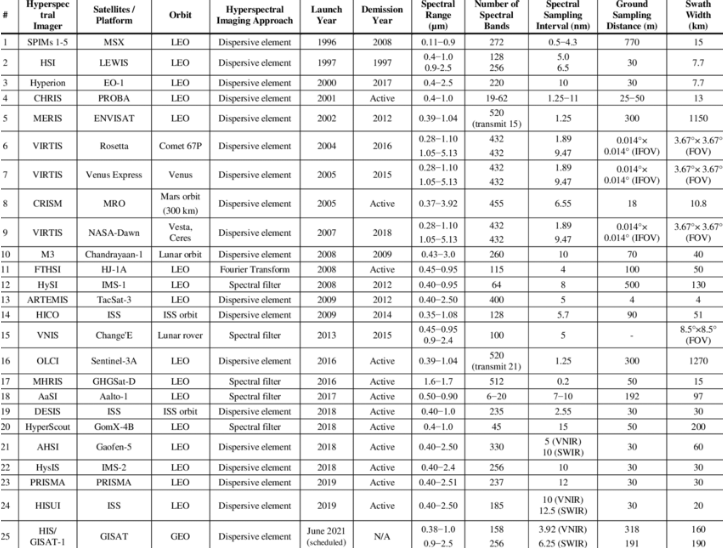
\includegraphics[width=0.9\textwidth]{img1.png}
\caption{Список спутниковых систем с гиперспектральной съемкой, запущенных до 2021 года.}
\label{fig::figure1}
\end{figure}

\subsection{Классификация задач анализа спутниковых снимков}

Задачи анализа спутниковых снимков могут быть классифицированы по различным критериям, включая типы данных, используемые методы анализа и цели исследования. Методы анализа будут подробно рассмотрены далее. В данном подразделе проведен поверхностный обзор различных целей исследования, а также дана общая классификация задач.

По целям исследования задачи можно разделить на следующие категории:

\begin{enumerate}
    \item Мониторинг различных объектов и процессов, таких как вырубка лесов, рост и созревание урожая, передвижение ледовых покровов, изменения в городской среде и других динамически изменяющийся объектов.
    \item Прогнозирование. Объектом исследования может являться урожайность, количество населения, а также различные стихийные бедствия.
    \item Исследование территорий. Поиск новых месторождений полезных ископаемых, подходящих мест для прокладки дорог или строительства сооружений являются одними из наиболее частых примеров.
\end{enumerate}

Стоит отметить, что хоть задачи и различаются достаточно сильно по целям исследования, при их декомпозиции они распадаются на 3 основные задачи:

\begin{itemize}
    \item Детекция (обнаружение) объектов на изображении;
    \item Классификация изображений;
    \item Семантическая сегментация.
\end{itemize}

Для каждой из этих задач разработаны и применяются отдельные методы решения, поэтому важно понимать специфику этих задач.

Детекция объектов на изображении – это процесс идентификации и локализации объектов на изображении. Эта задача является одной из ключевых в области компьютерного зрения и машинного обучения. Основные этапы детекции объектов:

\begin{enumerate}
    \item Сканирование изображения. На первом этапе алгоритм сканирует изображение, используя так называемое "скользящее окно" (sliding window). Это окно перемещается по изображению, и в каждом положении окна алгоритм пытается определить, есть ли на этом участке изображения объект, который нужно обнаружить.
    \item Выделение признаков. На этом этапе алгоритм анализирует каждый участок изображения, на котором может находиться объект, и выделяет признаки, которые помогут определить, есть ли на этом участке объект. Признаки могут включать в себя цвет, текстуру, форму и другие характеристики объекта.
    \item Классификация. После выделения признаков алгоритм классифицирует каждый участок изображения, определяя, есть ли на нем объект, и если да, то какого типа этот объект.
    \item Локализация. После того, как объекты были обнаружены и классифицированы, алгоритм определяет их точное положение на изображении. Это обычно делается путем определения ограничивающего прямоугольника (bounding box) вокруг каждого объекта.
\end{enumerate}

Задача классификации изображений заключается в отнесении входного изображения к одному или нескольким классам на основе его визуального содержимого. Основными этапами классификации изображений являются:

\begin{enumerate}
    \item Предварительная обработка изображения: Перед обучением модели все изображения приводятся к одному и тому же размеру. Также могут быть применены различные техники аугментации данных, такие как повороты, сдвиги, изменение масштаба и т.д., чтобы увеличить объем тренировочных данных и сделать модель более устойчивой к изменениям в входных данных.
    \item Извлечение признаков: На этом этапе из изображения извлекаются ключевые признаки, которые могут помочь в классификации. Это может быть сделано с помощью традиционных методов, таких как фильтры Габора или HOG (Histogram of Oriented Gradients), или с помощью сверточных нейронных сетей (Convolutional Neural Networks, CNN), которые могут автоматически извлекать и учить признаки из изображений.
    \item Классификация: После извлечения признаков эти данные подаются на вход классификатору, который может быть основан на различных методах машинного обучения, включая SVM (Support Vector Machines), случайные леса (Random Forests) или глубокие нейронные сети. Классификатор обучается на основе этих признаков, чтобы отнести каждое изображение к одному из предопределенных классов.
\end{enumerate}

Одной из наиболее перспективных и важных подзадач классификации является задача распознавания образов~\cite{20}.

Задача семантической сегментации является наиболее сложной из представленных. Семантическая сегментация изображений - это процесс разделения изображения на различные сегменты, где каждый сегмент представляет собой множество пикселей, которые принадлежат одному и тому же классу объектов. В отличие от задачи классификации изображений, где целью является определение класса всего изображения, или задачи детекции объектов, где целью является определение класса и положения отдельных объектов на изображении, семантическая сегментация стремится к классификации каждого пикселя изображения.

Основные этапы семантической сегментации схожи с этапами классификации за исключением заключительного шага. Он заменен на попиксельную классификацию, которая выполняется с помощь. сверточных нейронных сетей и др.

\subsection{Анализ методов обработки спутниковых снимков}

В последнее время с развитием области глубокого обучения появилось множество новых методов для обработки спутниковых снимков в дополнение к классическим методам. Классическими методами обработки спутниковых снимков в данной работе будут называться те, которые не содержат в себе продвинутых нейросетевых алгоритмов, таких, например, как глубокие сверточные нейронные сети (от англ. deep convolutional neural networks, CNN).

Классические методы можно разделить на 2 группы:

\begin{itemize}
    \item Методы, не связанные с обучением;
    \item Методы, основанные на обучении.
\end{itemize}

Методы, не связанные с обучением, в основном разрабатывались для решения задач детекции объектов. В них использовались различные подходы, например:

\begin{itemize}
    \item Вейвлет-анализ с несколькими разрешениями;
    \item Масштабно-инвариантное преобразование объектов;
    \item Модель набора слов для пространственного разреженного кодирования (от англ. spatial sparse coding bag-of-words) ~\cite{21}.
\end{itemize}

С развитием методов машинного обучения задачу детекции объектов стали рассматривать как задачу классификации и стали применять для ее решения различные подходы с использованием обучения:

\begin{itemize}
    \item Метод опорных векторов (от англ. Support Vector Machines);
    \item Модели гауссовой смеси (от англ. Gaussian Mixture Model);
    \item Квадратичный дискриминантный анализ;
    \item Решающие деревья, случайный лес (от англ. Random Forest).
\end{itemize}

Несмотря на развитие алгоритмов анализа спутниковых изображений, качество классификации для части изображений оставалось неадекватным. Это обуславливалось большим разнообразием пространственных и спектральных признаков изображений. Чтобы справиться с этой особенностью, были разработаны подходы, которые учитывали как пространственные, так и временные признаки изображения. Эти подходы основывались на таких методах, как:

\begin{itemize}
    \item Марковские случайные поля (от англ. Markov Random Field)~\cite{22};
    \item Условные случайные поля (от англ. Conditional Random Field)~\cite{23};
    \item Методы составного ядра (от англ. Composite Kernel Methods)~\cite{24}.
\end{itemize}

Описанные выше методы в настоящее время редко используются в практических задачах, поэтому не будем давать их подробное описание. На данные момент наиболее перспективными считаются методы, основанные на нейросетевых технологиях. Они тоже поддаются дополнительной классификации в зависимости от используемых подходов:

\begin{itemize}
    \item Сверточные нейронные сети. В настоящее время применяются различные модификации классической сверточной нейронной сети, такие как глубокие сверточные сети, сети с остаточными блоками (от англ. residual), 3-D сверточные сети. Последние широко применяются в анализе гиперспектральных изображений, так как позволяют учитывать сразу спектральные и пространственные признаки при применении операции свертки;
    \item Сети глубокого доверия. Состоят из композиции обучающих модулей, каждая из которых является ограниченной машиной Больцмана. Преимущество данной сети состоит в возможности “послойного” обучения ограниченных машин Больцама. Данные сети применяются для выделения скрытых признаков из распределения данных, оценки семантического расстояния между различными классами;
    \item Осцилляторные нейронные сети. Основная идея осцилляторной нейронной сети заключается в том, что нейроны могут быть представлены как осцилляторы, которые генерируют периодические сигналы. Эти сигналы могут быть синхронизированы с сигналами от других нейронов, что позволяет сети обрабатывать информацию и выполнять задачи по распознаванию образов. В осцилляторной нейронной сети, в общем случае, все нейроны полностью связаны (fully connected). Это означает, что каждый нейрон может получать сигналы от всех остальных нейронов в сети;
    \item Многослойные автоэнкодеры. Они состоят из двух основных частей: кодировщика (encoder), который преобразует входные данные в некоторое скрытое представление, и декодера (decoder), который восстанавливает данные из этого скрытого представления. Для задач обработки гиперспектральных изображений интерес представляет распределение признаков в скрытом представлении. Его еще называют латентным пространством (от англ. latent space). Выбор признаков из данного пространства помогает уменьшить размерность данных, при этом сохранив ключевую информацию, заключенную в изображении;
    \item Визуальные трансформеры (от англ. visual transformers). Это модели машинного обучения, которые применяют архитектуру трансформера, изначально разработанную для обработки естественного языка, к задачам компьютерного зрения. Визуальные трансформеры начинают с разделения входного изображения на решетку небольших патчей или "визуальных токенов". Эти патчи затем линеаризуются и обрабатываются с использованием трансформера. Трансформер состоит из нескольких слоев, каждый из которых содержит два основных компонента: механизм внимания и полносвязные сети (от англ. feed-forward networks, FFN). Механизм самовнимания позволяет модели учесть контекст каждого визуального токена, учитывая все остальные токены, а FFN обеспечивают дополнительную обработку. В отличие от традиционных сверточных нейронных сетей (от англ. convolutional neural networks, CNN), которые обрабатывают изображения с использованием локальных сверток, визуальные трансформеры обрабатывают все визуальные токены одновременно, что позволяет им учесть глобальные зависимости между различными частями изображения~\cite{25}.
\end{itemize}

\subsection{Выводы по разделу 1}
\begin{enumerate}
    \item Проведен обзор различных типов изображений, получаемых со спутников.
    \item Рассмотрены различные типы задач, встречающиеся в процессе анализа спутниковых снимков.
    \item Проанализированы различные методы и алгоритмы обработки снимков, в том числе с использованием новейших достижений в области нейросетевых технологий.
\end{enumerate}

\section{Осцилляторные нейронные сети}\label{Sect::onn}

\subsection{Исследование входных данных при разработке осцилляторных нейронных сетей}

Этап предварительного исследования входных данных является важной частью процесса разработки искусственных нейронных сетей, в частности осцилляторных нейронных сетей (ОНС). В данном параграфе будут подробно рассмотрены только те аспекты входных данных, которые непосредственно влияют  на выбор архитектуры ОНС, процесс обучения и полученный результат в контексте задачи обработки гиперспектральных изображений.

Рассмотрим некоторые особенности осцилляторных нейронных сетей:

\begin{itemize}
    \item Информация в ОНС запоминается на основе фаз ее составных элементов, осцилляторов;
    \item Размер ОНС растет пропорционально количеству паттернов или объектов, которые могут быть классифицированы или сегментированы ~\cite{26};
    \item Способность ОНС к адаптации, проявляющаяся в модификации параметров (весов) элементов или связей в качестве реакции на внешнюю среду.
\end{itemize}

Учитывая вышеизложенные особенности ОНС, а также специфику гиперспектральных изображений, описанную в блоке 1.1, стоит обратить внимание на следующие ограничения параметров входных данных:

\begin{itemize}
    \item Невысокое количество различных типов целевых объектов;
    \item Не учитывается распределение одновременно пространственных и спектральных признаков (при использовании классического варианта ОНС);
    \item При высокой сложности целевых объектов потребуется использование многослойных ОНС, что может заметно увеличить их размер и время работы.
\end{itemize}

Принимая во внимание данные ограничения, можно сузить область эффективного применения ОНС, исключив из нее, в общем случае, задачи семантической сегментации. В частном случае, при малом количестве типов объектов на снимке, ОНС применимы к этому типу задач.

Несмотря на некоторые ограничения, ОНС могут обрабатывать широкий набор входных данных. Кроме того, они допускают изменение вида или формы целевого объекта при незначительной потере точности, что позволяет несколько расширить множество входных данных.

\subsection{Архитектуры осцилляторных нейронных сетей}

Для успешного построения модели ОНС необходимо определить модель ее составной части, нейрона (осциллятора). Рассмотрим наиболее распространенные модели осцилляторов:

\begin{enumerate}
    \item Модифицированный осциллятор Ван дер Поля. Он представляет собой релаксационный осциллятор, его динамика определяется двумя связанными переменными х и у и подчиняется двумерной динамической системе
        \begin{equation}\label{eq:1}
            \begin{split}
                &\dot{x} = f(x,y) + S + I + \eta, \quad f(x,y) = 3x - x^3 + 2 - y,\\
                &\dot{y} = \epsilon g(x, y), \qquad \qquad \qquad g(x, y) = \alpha(1 + \tanh(\frac{x}{\beta})) - y,
            \end{split} 
        \end{equation}где $S$ определяет влияние (общий вклад) связей в ОНС, $I$ представляет собой входные данные (определяется характеристиками изображения), $\eta$ это Гауссовый шум, и $\epsilon,\alpha,\beta$ это положительно определенные параметры, контролирующие форму предельного цикла осциллятора~\cite{27};
    \item Осциллятор предельного цикла. Данный осциллятор описывается 2-мя нейронами, возбуждающим и тормозным. Его управляющая динамическая система может быть выписана в следующем виде
        \begin{equation}\label{eq:2}
            \begin{split}
                &\dot{u} = -u + \alpha h(u) - g(v) + I^+\\
                &\dot{v} = -v + \beta h(u) + I^-,
            \end{split} 
        \end{equation}где $u$ и $v$ отвечают за "потенциалы" возбуждающего и тормозного нейрона соответсвенно, $h(u)$ -- это фукнция активации возбуждающего нейрона (в данном случае используется сигмоида или схожие с ней функции), $g(v)$ -- функция активации тормозного нейрона (используется любая монотонная неубывающая функция) и $I^\pm$ отражают признаки входных данных для возбуждающего и тормозного нейрона соответственно.
        Стоит заметить, что динамическая система обладает устойчивым предельным циклом, при условии, что значения признаков входных данных $I^\pm$ принадлежат ограниченному интервалу.
    \item Модифицированный осциллятор Гинзбурга-Ландау. Осциллятор задается двумя значениями $u_1, u_2 \in \mathbb{R} $. Тогда двумерная динамическая управляющая система представляется в виде одного уравнения с использование комплексной переменной $u = u_1 + i u_2,\ u \in \mathbb{C}$
        \begin{equation}\label{eq:3}
            \dot{u} = f(u) + g(I), \quad f(u) = (p^2_0 + i\omega - |u - c|^2)(u - c),
        \end{equation}где $p_0$ и $c = c_x + ic_y$ константы, задающие параметры предельного цикла осциллятора при $g(I) = 0$. Этот предельный цикл можно описать как круг радиуса $p_0$, расположенный в комплексной плоскости $(u_1, u_2)$ с координатами $(c_x, c_y)$ при $g(I) = 0$. $\omega$ это собственная частота осциллятора. 
        Функция $g(I)$ зависит от признаков входного изображения. При этом она контролирует размер и местоположение предельного цикла осциллятора в комплексной плоскости $(u_1, u_2)$. По размеру цикла можно определять яркость $I$ пикселя, за который отвечает осциллятор, больше чем предопределенно заданное пороговое значение $I^*$.
        В этом случае мы можем считать состояние осциллятора как "активное". В противном случает предельный цикл осциллятора сходится в точку стабилизации (стабильный фокус). Состояние данного осциллятора определяется как "пассивное" или "неактивное".
\end{enumerate}

Далее перейдем к описанию самих моделей.

Сеть фазовых осцилляторов Курамото-Сакагучи. Данная модель может применяться как в сетях с глобальными или локальными связями, так и в системах с центральным элементов [26]. В общем случае модель взаимодействия фазовых осцилляторов можно описать уравнением~(\ref{eq:4}) (модель Курамото), а в частном случае (функция взаимодействия является синусоидальной, а тажке добавлены фазовые сдвиги) уравнением~(\ref{eq:5}) (Модель Курамото-Сагучи)
\begin{equation}\label{eq:4}
    \frac{\partial \theta_i}{\partial t} = \omega_i + \sum_{j = 1}^{n}K_{ij} f(\theta_j - \theta_i), \ i = 1,...,n,
\end{equation}
\begin{equation}\label{eq:5}
    \frac{\partial \theta_i}{\partial t} = \omega_i + \sum_{j = 1}^{n}K_{ij} \sin(\theta_j - \theta_i - \alpha_{ij}), \ i = 1,...,n,
\end{equation}где $\theta_i$ - фаза $i$-го осциллятора, $\omega_i$ - собственная частота осциллятора, $K_ij$ можно интерпретировать как "веса" направленных связей между осцилляторами $j$ и $i$ (как сильно осциллятор $j$ влияет на осциллятор $i$). $f$, в общем случае периодическая нечетная фунция, определяет взаимодействие между осцилляторами.

Для описания модель с центральным осциллятором (ЦО) потребуется 2 уравнения
\begin{equation}\label{eq:6}
    \frac{\partial \theta_0}{\partial t} = \omega_0 + \frac{A}{n} \sum_{j = 1}^{n}f(\theta_j - \theta_0 + \gamma),
\end{equation}
\begin{equation}\label{eq:7}
    \frac{\partial \theta_i}{\partial t} = \omega_i + B g(\theta_0 - \theta_i + \delta), \ i = 1,...,n,
\end{equation}где $A$, $B$ также можно интерпретировать как "веса" (параметры взаимодействия).
В уравнении~(\ref{eq:6}) записана модель для ЦО. Через этот осциллятор происходят все взаимодействия в системе. Уравнение~(\ref{eq:7}) задает модель периферических осцилляторов (ПО).
Следует отметить, что полученная модель для ЦО и ПО дает возможность выполнять подбор параметров для достижения определенного режима работы системы (полная или частичная синхронизация с ЦО)

Сеть фазовых осцилляторов Хонг-Строгаца. Данная модель является обобщением модели с ЦО и ПО в том случае, если присутствует синхронизирующее воздействие от ПО к ЦО и десинхронихирующем воздействии от ЦО к ПО.

Она состоит из двух популяций фазовых осцилляторов. Осцилляторы первой популяции получают из входных данных только синхронизирующие воздействия,
 а осцилляторы второй группы только десинхронизирующие воздействия соответсвенно. В результате такой организации взаимодействия между осцилляторами представители первой группы стремятся синхронизироваться с осцилляторами, которые оказывают на них воздействие, а вторая группа наоборот, старается работать в противофазе с воздействующими на них осцилляторами. Назовем первую группу фазовых осцилляторов конформистами, а вторую нонконформистами.

Модель Хонг-Строгаца можно описать формулами, схожими с~(\ref{eq:4}). Обозначим весь набор осцилляторов как $J$. Весь набор состоит из $n$ элементов. Пусть $J_1, J_2$ -- группы конформистов и нонконформистов, соответственно. Теперь запишем динамику модели
\begin{equation}\label{eq:8}
    \frac{\partial \theta_i}{\partial t} = \omega + \frac{A}{n} \sum_{j = 1}^{n}f(\theta_j - \theta_0 + \gamma),
\end{equation}
\begin{equation}\label{eq:8}
    \frac{\partial \theta_i}{\partial t} = \omega + \frac{A}{n} \sum_{j = 1}^{n}f(\theta_j - \theta_0 + \gamma),
\end{equation}где $k_1, k_2$, аналогично предыдущим моделям, параметры ("веса") связей. При этом $k_1 > 0,\ k_2 < 0$, что отражает различие в принципе работы двух групп осцилляторов.

После рассмотрения базовых моделей ОНС перейдем к построению многослойной архитектуры ОНС,
которая сможет решать задачу сегментации целевых объектов на гиперспектральном изображении.
Для решения этой задачи возможны два подхода, которые будут влиять на архитектуру многослойной ОНС.
Обозначим первый подход как базовый, а второй как продвинутый:

\begin{enumerate}
    \item Априорный выбор значимых (в рамках признаков целевого объекта) спектральных каналов и применение трехслойной модели сегментации для 2-х мерного изображения.
    \item Добавление спектральных каналов как 3-ую размерность во входные данные и модификация модели из 1-го пункта для обработки 3-х мерных изображений.
\end{enumerate}

Для базового подхода модель будет состоять из модуля селективного внимания, модуля выделения границ объекта (контуров) и модуля сегментации объектов.
(написать побольше про модули)

\subsection{Обучение осцилляторных нейронных сетей}

В силу того, что ОНС по своей архитектуре являются рекуррентными нейронными сетями (РНС), то для их обучения могут применяться обучающие правила и подходы, разработанные для обучения без учителя. В данном параграфе будут рассмотрены обучающие правила Хеббиана, Сторки, а также принцип “победитель получает все” (ППВ).

Правило Хеббиана. Наиболее простая форма правила Хеббиана может быть описана как процесс измения (эволюции) матрицы связи $\hat{W} = [W_{ij}]$ при в условиях дискретного времени:
\begin{equation}\label{eq:9}
    W_{ij}(t) = W_{ij}(t-1) + \Delta W_{ij}(t), \quad \Delta W_{ij}(t) = \eta y_i(t) x_j(t), 
\end{equation}где $x_{j}(t)$ -- состояние входного нейрона, $y_i(t)$ -- состояние выходного нейрона и $\eta \ (\eta \geq 0)$ параметр, отвечающий за скорость обучения (от англ. learning rate).

Правило~(\ref{eq:9}) имеет недостаток ввиде экспоненциального увеличения состояния $y_i(t)$ из-за повторяющийся обучающих серий, примененных к входному нейрону $x_{j}(t)$. Поэтому были предложены улучшенные версии этого правила, например:

\begin{equation}\label{eq:10}
    \frac{\partial \hat{W}}{\partial t} = \eta (\mathbf{y x^T} - \mathbf{y^T y} \hat{W}).
\end{equation}Данное правило записано в условиях непрерывного времени.

Далее рассмотрим специальный вариант правила Хеббиана, а именно "соревновательное обучение". Смылс этого правила состоит в том, что выходные нейроны соревнуются между собой за входные нейроны.
Выходной нейрон, который показал наибольший уровень активации, побеждает и его связь изменяется в то время как остальные нейроны остаются без изменений. Такую стратегию называют принципом "победитель получает все" (от англ. winner-takes-all) и он будет подробнее рассмотрен далее.
Соревновательный алгоритм обучения, который подходит для использования в многослойных рекуррентных нейронных сетях может быть формализован следующим образом:
 \begin{equation}\label{eq:11}
    \Delta W_{ij}(t) = 
    \begin{cases}
        \eta[x_i(t) - W_{ij}(t)] & \texttt{если j-ый нейрон выигрывает} \\
        0 & \texttt{иначе}
    \end{cases}
\end{equation}

Существенной особенностью любого обучения без учителя (в частности, обучения Хеббиана и его обобщений) является автоматический,
самоорганизующийся характер изменения структуры сетевой связности.

Правило Сторки. Данное правило схоже с правилом Хеббиана, но позволяется хранить больше запомненных образов и более устойчиво к зависимым образам~\cite{28}. 
Запишем форулу для этого правила в условиях дискретного времени:
\begin{equation}\label{eq:12}
    W_{ij}(t) = W_{ij}(t-1) + \frac{1}{n} (y_i(t) x_j(t) - y_i(t) h_{ji}(t) - h_{ij}(t) x_j(t))
\end{equation}
\begin{equation}\label{eq:13}
    h_{ij}(t) = \sum_{k = 1, k \neq i,j}^{n} W_{ik}(t-1) y_{k} (t)
\end{equation}

Принцип ППВ. Принцип "победитель получает все" (от англ. Winner-Take-All, WTA) в контексте обучения нейронных сетей относится к ситуации, когда только один нейрон или группа нейронов активируется в ответ на входные данные. Этот нейрон или группа нейронов считается "победителем" и получает возможность обучаться на этих данных, в то время как остальные нейроны остаются неактивными.
Этот принцип часто используется в моделях, основанных на конкуренции, где нейроны соревнуются за право реагировать на входные данные. Например, в самоорганизующихся картах Кохонена, нейроны соревнуются за то, чтобы стать "победителем" , и только победитель обновляет свои веса в процессе обучения.

Для реализаци модулей внимания, упомянутых в предыдущем разделе, требуется разработать правило, которое учитывало бы особенности биологической модели внимания. 
В этом случае принцип ППВ отлично подходит на эту роль, так как он обеспечивает фокусировку внимания на одном объекте. При этом случаи отсутсвия фокусировки (победителя не оказывается) возникают достаточно редко.
Если перенести этот принцип на разработанную модель с ЦО и ПО, то он обеспечивает, что синхронизирован с ЦО будет лишь один ПО. 
Следует отметить, что для реализации принципа ППВ необходимо применять его в сети с динамическими (адаптирующимися) параметры. В нашем случае собственная частота осциллятора, а также величины связи между нейронами будут динамическими переменными.
Тогда динамику модели можно описать следующими уравнениями
\begin{equation}\label{eq:14}
    \frac{\partial \theta_0}{\partial t} = \omega_0 + \frac{1}{n} \sum_{i = 1}^{n}a_i f(\theta_i - \theta_0),
\end{equation}
\begin{equation}\label{eq:15}
    \frac{\partial \theta_i}{\partial t} = \omega_i + b g(\theta_0 - \theta_i),\quad i = 1,\ldots,n,
\end{equation}
\begin{equation}\label{eq:16}
    \frac{\partial \omega_0}{\partial t} = \frac{\alpha}{n} \sum_{i = 1}^{n}a_i f(\theta_i - \theta_0),
\end{equation}
\begin{equation}\label{eq:17}
    \frac{\partial a_i}{\partial t} = \beta(-a_i + c + \gamma h(\theta_i - \theta_0)), \quad i = 1,\ldots,n,
\end{equation}где $\theta = (\theta_0, \theta_1, \ldots, \theta_n),\ \omega_0 \in \mathbb{R},\ a = (a_1, \ldots, a_n) \in \mathbb{R}^n$ -- переменные. Уравнение~(\ref{eq:16}) задает адаптапцию собственной частоты ЦО по направлению к его текущей частоте, $\alpha$ -- параметр скорости адаптации. Параметр $\beta$ отвечает за скорость изменения амплитуд, а параметры $c$ и $c + \gamma$ задают минимальный и максимальный уровень амплитуды ПО. 

Генетический алгоритм. Это метод оптимизации и поиска решений, который имитирует процессы естественной эволюции, такие как наследование, мутация, отбор и кроссовер (рекомбинация).

Генетический алгоритм начинается с генерации начальной популяции решений, обычно представленных в виде хромосом или строк кода. Каждое решение оценивается с помощью функции приспособленности, которая определяет, насколько хорошо оно решает поставленную задачу.
Затем алгоритм входит в цикл, который повторяется до тех пор, пока не будет достигнут критерий остановки, например, достаточно хорошее решение или определенное количество поколений. В каждом поколении происходят следующие шаги~\cite{29}:
\begin{enumerate}
    \item Отбор. "Особи" отбираются для создания новго поколения. Отбор происходит на основании значения функции фитнеса. Эта функция показывает, на сколько пригодна данная "особь" для решения конкретной задачи. Выбор корректной функции фитнеса является одним из ключевых этапов разработки генетического алгоритма. Для отбора есть несколько различных методов, например рулетка или турнирный.
    \item Кроссинговер (рекомбинация). С помощью двух ДНК (генов) выбранных "особей" создается новая особь с измененным набором генов. Полученные ей гены зависят от методов, которыми осуществяется рекомбинация. Различают дискретную рекомбинацию и кроссинговер. Кроссинговер, в свою очередь, делится на одноточечный, двухточечный и многоточечный. Также важную роль играет способ выбора родителей. Их можно выбрать случайным образом, либо наиболее близких или далеких по набору генов. Расстояние между наборами генов считается по метрике, применимой к пространству ДНК "особей".
    \item Мутация. Это заключительный этап в рамках одного поколения. Мутация позволяет существенно изменить набор генов отдельных особей. Это добавляет вариативность в популяцию и помогает преодолевать локальные минимумы. Стоит отметить, что существует множество способов выбора особей для мутации, а также самих методов изменения генов.
\end{enumerate}
В контексте нашей задачи генетический алгоритм обладает наиболее широкой областью применения, но проигрывает приведенным правилам и принципам в собласти обучения модулей ОНС. 
Поэтому будет рассмотрена возможнось применения генетического алгоритма для выбора спектральных каналов, для которых будет производится дальнейшая обработка.

\begin{listing}[!htt]
    \caption{Обобщенный класс модели}
    \label{lst:detection_model}
    \begin{minted}[frame=single, breaklines, fontsize = \footnotesize, linenos]{python}
    class Model(nn.Module):
        def __init__(self, model_config: dict):
            """ model init
            Args:
                model_config (dict): backbone, neck and head params
            """
            super().__init__()
            self.backbone = build_backbone(model_config.backbone)
            self.neck = build_neck(model_config.neck)
            self.head = build_head(model_config.head)
    
        def forward(self, x):
            backbone_out = self.backbone(x)
            neck_out = self.neck(backbone_out)
            y = self.head(neck_out)
            return y
    \end{minted}
\end{listing}
    

\subsection{Выводы по разделу 2}

\begin{enumerate}
    \item 
\end{enumerate}

\anonsection{ЗАКЛЮЧЕНИЕ} %\anonsection{Заключение}

Все супер пупер работает

\renewcommand\refname{СПИСОК ИСПОЛЬЗОВАННЫХ ИСТОЧНИКОВ}
\renewcommand{\mkgostheading}[1]{#1}
\renewcommand*{\newblockpunct}{\addperiod\addnbspace\textendash\space\bibsentence}
\renewcommand*{\bibrangedash}{\text{\textendash}}

% Список литературы
\clearpage
% \bibliographystyle{ugost2008s} %utf8gost71u.bst} %utf8gost705u} %gost2008s}
{\catcode`"\active\def"{\relax}
\addcontentsline{toc}{section}{\protect\numberline{}\refname}%
% \bibliography{biblio} %здесь ничего не меняем, кроме, возможно, имени bib-файла
\printbibliography
}

\end{document}